\section{$\rho_1$ is not a 4-transposition}

\paragraph{}
By Lemma~\ref{min-4-trans}, at least one 4-transposition is needed. It cannot be at the $\rho_1$ position ($\rho_3$ is impossible too by duality). Therefore, $\rho_2$ must be the 4-transposition.

\paragraph{}
In this case, no generator can be omitted. Thus, if one generator is removed, the remaining group would be a sggi of rank 4 with a single 4-transposition but Lemma~\ref{min-4-trans} proved that it cannot generate $A_{11}$.

\begin{theorem}
  The only permutation representation graph of rank 5 on 11 points are those displayed in appendix~\ref{monodromy-5} (p.~\pageref{monodromy-5}).
\end{theorem}

\begin{proof}
  All the possibilities for the permutation representation graphs will be built. The graph with only the 4-transposition $\rho_2$ looks like this:

  \begin{figure}[H]
    \begin{center}
      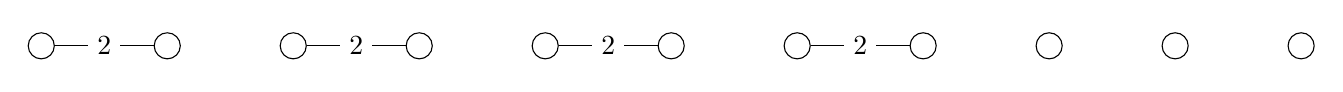
\begin{tikzpicture}[scale=.8]

        \begin{scope}[every node/.style={circle,draw}]
          \node (1)  at (-2,0)  {};
          \node (2)  at (0,0)  {};
          \node (3)  at (2,0)  {};
          \node (4)  at (4,0)  {};
          \node (5)  at (6,0)  {};
          \node (6)  at (8,0)  {};
          \node (7)  at (10,0)  {};
          \node (8)  at (12,0)  {};
          \node (9)  at (14,0)  {};
          \node (10)  at (16,0)  {};
          \node (11)  at (18,0)  {};
        \end{scope}

        \begin{scope}[every node/.style={fill=white}]

          \begin{scope}[every edge/.style={draw}]
            \path (1)  edge node {$2$} (2);
            \path (3)  edge node {$2$} (4);
            \path (5)  edge node {$2$} (6);
            \path (7)  edge node {$2$} (8);
          \end{scope}
        \end{scope}

      \end{tikzpicture}
      \caption{[1, 5, 1010, 232, 381]}
    \end{center}
  \end{figure}

\paragraph{}
If the involutions $\rho_0$ and $\rho_4$ are added to the graph, they must commute with $\rho_2$ and so the only possibilities are:
\begin{enumerate}
  \item A double edge with $\rho_2$ and link two currently fixed points.
  \item Two double edges with $\rho_2$.
  \item An alternating square with $\rho_2$.
\end{enumerate}

\paragraph{}
Since there is only one 4-transposition, there are only 12 edges to link 11 points, 2 more than the minimum. Thus if a edge is added, it must link two distinct components, expect two times. Those two edges are called "joker" edges. When an alternating square is built, one of those edge is used, it is the same if a double edge is built.

\paragraph{}
Among the three possibilities, the second is impossible because, if it is used, even once, it uses both "joker" edges and it is not possible to place the other involution.

\paragraph{}
The same choice cannot be made for $\rho_0$ and $\rho_4$. The first proposition cannot be used twice because it links two fixed points. There are only three of them and so it cannot be used two times.

\paragraph{}
If the third proposition is used twice, there are two alternating squares. If those squares does not share a vertex, they cannot be linked. Thus one square must be linked to the rest of the graph by a $\rho_1$ edge and the other by a $\rho_3$. But those two edges cannot be linked because all $\rho_2$ have already be used and no more alternating square or double edges cannot be used.

\paragraph{}
If the two squares share an edge, a $\rho_0$ and a $\rho_4$ edge are next to each other but that is impossible by Lemma~\ref{0-4-no-share}.

\paragraph{}
The two squares cannot share all their vertices because it will not be able to be connected two the rest of the graph.

\paragraph{}
Thus one of the involution must build an alternating square and the other must build a double edge and links two fixed points. By duality, only the case where $\rho_4$ makes an alternating square will be considered and the other doubles an edge and links two fixed points.

\begin{figure}[H]
  \begin{center}
    \begin{tikzpicture}[scale=.8]

      \begin{scope}[every node/.style={circle,draw}]
        \node (1)  at (12,2)  {};
        \node (2)  at (12,0)  {};
        \node (3)  at (14,2)  {};
        \node (4)  at (14,0)  {};
        \node (5)  at (6,0)  {};
        \node (6)  at (4,0)  {};
        \node (7)  at (10,0)  {};
        \node (8)  at (8,0)  {};
        \node (9)  at (2,0)  {};
        \node (10) at (0,0)  {};
        \node (11) at (16,0) {};
      \end{scope}

      \begin{scope}[every node/.style={fill=white}]

        \begin{scope}[every edge/.style={draw}]
          \path (9)  edge node {$0$} (10);
          \path (7)  edge[bend right=30] node {$0$} (8);
          \path (1)  edge node {$2$} (2);
          \path (3)  edge node {$2$} (4);
          \path (5)  edge node {$2$} (6);
          \path (7)  edge[bend left=30] node {$2$} (8);
          \path (1)  edge node {$4$} (3);
          \path (2)  edge node {$4$} (4);
        \end{scope}
      \end{scope}

    \end{tikzpicture}
    \caption{The graph with only $\rho_0$ and $\rho_2$}
  \end{center}
\end{figure}

\paragraph{}
Now that all of our "joker" edges has been used, every other edge must link two different connected components of the graph.

\paragraph{}
Now the $\rho_3$ edge will be placed. It cannot be adjacent to the component consisting of the single $\rho_0$ edge or to the double edge. There are only three components that can be adjacent to such edge. Thus there are three places for two edges. The component that we are currently building must be linked to the rest of the graph by $\rho_1$ edges and a $\rho_1$ edge can only be connected to the single $\rho_2$ edge. This edge must so be connected by only one $\rho_3$ edge. The same applies for the fixed point that cannot be connected two times, otherwise two $\rho_3$ edges will share this vertex.

\paragraph{}
The square must thus be connected twice. There are three possibilities: the two connected vertices can be opposed or adjacent and, in this case, separated by a $\rho_1$ or a $\rho_3$ edge. This does not influence the position of the $\rho_1$ edges. It is possible to continue building the graph without having to deal with cases. Here is one of the possible graphs:

\begin{figure}[H]
  \begin{center}
    \begin{tikzpicture}[scale=.8]

      \begin{scope}[every node/.style={circle,draw}]
        \node (1)  at (0,2)  {};
        \node (2)  at (0,0)  {};
        \node (3)  at (-2,2)  {};
        \node (4)  at (-2,0)  {};
        \node (5)  at (-6,0)  {};
        \node (6)  at (-4,0)  {};
        \node (7)  at (-10,0)  {};
        \node (8)  at (-8,0)  {};
        \node (9)  at (-14,0)  {};
        \node (10) at (-12,0)  {};
        \node (11) at (2,0) {};
      \end{scope}

      \begin{scope}[every node/.style={fill=white}]

        \begin{scope}[every edge/.style={draw}]
          \path (9)  edge node {$0$} (10);
          \path (7)  edge[bend right=30] node {$0$} (8);
          \path (1)  edge node {$2$} (2);
          \path (3)  edge node {$2$} (4);
          \path (5)  edge node {$2$} (6);
          \path (7)  edge[bend left=30] node {$2$} (8);
          \path (2)  edge node {$3$} (11);
          \path (4)  edge node {$3$} (6);
          \path (1)  edge node {$4$} (3);
          \path (2)  edge node {$4$} (4);
        \end{scope}
      \end{scope}

    \end{tikzpicture}
    \caption{One of the graphs after placing $\rho_3$ edges}
  \end{center}
\end{figure}

\paragraph{}
Now the two edges of $\rho_1$ must be placed, the component containing the alternating square must be attached by its left end, the one that ends with a $\rho_2$ edge. The first two components must be linked together. The first component can be attached in two ways depending on the end choose to be attached. Here is one of the graphs:

\begin{figure}[H]
  \begin{center}
    \begin{tikzpicture}[scale=.8]

      \begin{scope}[every node/.style={circle,draw}]
        \node (1)  at (0,2)  {};
        \node (2)  at (0,0)  {};
        \node (3)  at (-2,2)  {};
        \node (4)  at (-2,0)  {};
        \node (5)  at (-6,0)  {};
        \node (6)  at (-4,0)  {};
        \node (7)  at (-10,0)  {};
        \node (8)  at (-8,0)  {};
        \node (9)  at (-14,0)  {};
        \node (10) at (-12,0)  {};
        \node (11) at (2,0) {};
      \end{scope}

      \begin{scope}[every node/.style={fill=white}]

        \begin{scope}[every edge/.style={draw}]
          \path (9)  edge node {$0$} (10);
          \path (7)  edge[bend left=30] node {$0$} (8);
          \path (5)  edge node {$1$} (8);
          \path (7)  edge node {$1$} (10);
          \path (1)  edge node {$2$} (2);
          \path (3)  edge node {$2$} (4);
          \path (5)  edge node {$2$} (6);
          \path (7)  edge[bend right=30] node {$2$} (8);
          \path (2)  edge node {$3$} (11);
          \path (4)  edge node {$3$} (6);
          \path (1)  edge node {$4$} (3);
          \path (2)  edge node {$4$} (4);
        \end{scope}
      \end{scope}

    \end{tikzpicture}
    \caption{One sggi on $A_{11}$ of rank 5}
  \end{center}
\end{figure}

\paragraph{}
There are 6 possible graphs but only one was built. The construction of the five remaining graphs is left to the reader. He can check that the graphs built match the graphs of appendix~\ref{monodromy-5}.

\end{proof}


\begin{theorem}
  None of the groups represented by the graphs of appendix~\ref{monodromy-5} are C-groups.
\end{theorem}

\begin{proof}
  By the definition of a C-group, it is sufficient to find two subsets of generators $S_1$ and $S_2$ such that $\Gamma_{S_1} \cap \Gamma_{S_2} \neq \Gamma_{S_1 \cap S_2}$.

  \paragraph{}
  This proof is inspired by the section 4 of~\cite{leemansTransactions}.

  \paragraph{}
  In this case, they will be choose $S_1 = \{\rho_1, \rho_2\}$ and $S_2 = \{\rho_2, \rho_3, \rho_4\}$. Here $S_1 \cap S_2 = \{\rho_2\}$ and so $\Gamma_{S_1 \cap S_2} = \Gamma_{\rho_2}$ is a cyclic group of order 2. Hence, $\rho_2$ is an involution.

  \paragraph{}
  $S_1$ will be studied more deeply, only the $\rho_1$ and $\rho_2$ edges are kept in all the possible graphs. There are only two possible graphs:

  \begin{figure}[H]
    \begin{center}
      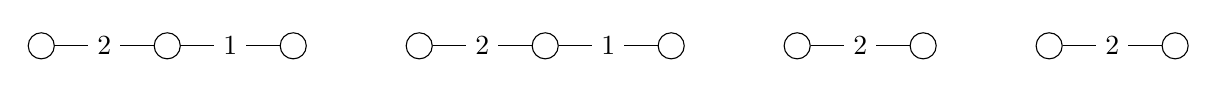
\begin{tikzpicture}[scale=.8]

        \begin{scope}[every node/.style={circle,draw}]
          \node (1)  at (-2,0)  {};
          \node (2)  at (0,0)  {};
          \node (3)  at (2,0)  {};
          \node (4)  at (8,0)  {};
          \node (5)  at (6,0)  {};
          \node (6)  at (4,0)  {};
          \node (7)  at (12,0)  {};
          \node (8)  at (10,0)  {};
          \node (9)  at (16,0)  {};
          \node (10) at (14,0)  {};
        \end{scope}

        \begin{scope}[every node/.style={fill=white}]

          \begin{scope}[every edge/.style={draw}]
            \path (2)  edge node {$1$} (3);
            \path (4)  edge node {$1$} (5);
            \path (1)  edge node {$2$} (2);
            \path (5)  edge node {$2$} (6);
            \path (7)  edge node {$2$} (8);
            \path (9)  edge node {$2$} (10);
          \end{scope}
        \end{scope}

      \end{tikzpicture}
      \caption{First possibility for $\Gamma_{S_1}$}
    \end{center}
  \end{figure}

  \begin{figure}[H]
    \begin{center}
      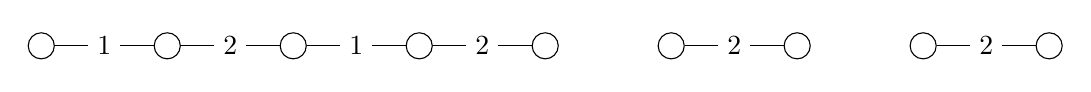
\begin{tikzpicture}[scale=.8]

        \begin{scope}[every node/.style={circle,draw}]
          \node (2)  at (0,0)  {};
          \node (3)  at (2,0)  {};
          \node (4)  at (4,0)  {};
          \node (5)  at (6,0)  {};
          \node (6)  at (8,0)  {};
          \node (7)  at (12,0)  {};
          \node (8)  at (10,0)  {};
          \node (9)  at (16,0)  {};
          \node (10) at (14,0)  {};
        \end{scope}

        \begin{scope}[every node/.style={fill=white}]

          \begin{scope}[every edge/.style={draw}]
            \path (2)  edge node {$1$} (3);
            \path (4)  edge node {$1$} (5);
            \path (3)  edge node {$2$} (4);
            \path (5)  edge node {$2$} (6);
            \path (7)  edge node {$2$} (8);
            \path (9)  edge node {$2$} (10);
          \end{scope}
        \end{scope}

      \end{tikzpicture}
      \caption{Second possibility for $\Gamma_{S_1}$}
    \end{center}
  \end{figure}

  \paragraph{}
  In the first graph, the permutation $(\rho_1 \rho_2)^2 \rho_1$ lets the points of the two isolated edges fixed because the permutation uses $\rho_2$ an even number of times. The points only linked by $\rho_1$ edges remain fixed too. But the point linked by $\rho_2$ edges in the big components are swapped. So it is possible to permute only two $\rho_2$ edges without touching the two others.

  \paragraph{}
  In the second graph, $(\rho_1\rho_2)^4 \rho_1$ gives the same result.

  \paragraph{}
  Now, let's study $S_2$, the disposition of the edges alongside the alternating square is very important. Therefore there are 3 possibilities:

  \begin{figure}[H]
    \begin{center}
      \begin{tikzpicture}[scale=.8]

        \begin{scope}[every node/.style={circle,draw}]
          \node (1)  at (-2,0)  {};
          \node (2)  at (0,0)  {};
          \node (5)  at (2,0)  {};
          \node (6)  at (4,0)  {};
          \node (7)  at (6,0)  {};
          \node (8)  at (6,2)  {};
          \node (9)  at (8,2)  {};
          \node (10) at (8,0)  {};
          \node (11) at (10,0) {};
        \end{scope}

        \begin{scope}[every node/.style={fill=white}]

          \begin{scope}[every edge/.style={draw}]
            \path (1)  edge node {$2$} (2);
            \path (5)  edge node {$2$} (6);
            \path (7)  edge node {$2$} (8);
            \path (9)  edge node {$2$} (10);
            \path (6)  edge node {$3$} (7);
            \path (10) edge node {$3$} (11);
            \path (7)  edge node {$4$} (10);
            \path (8)  edge node {$4$} (9);
          \end{scope}
        \end{scope}

      \end{tikzpicture}
      \caption{First possibility for $\Gamma_{S_2}$}
    \end{center}
  \end{figure}

  \begin{figure}[H]
    \begin{center}
      \begin{tikzpicture}[scale=.8]

        \begin{scope}[every node/.style={circle,draw}]
          \node (1)  at (-2,0)  {};
          \node (2)  at (0,0)  {};
          \node (5)  at (2,0)  {};
          \node (6)  at (4,0)  {};
          \node (7)  at (6,0)  {};
          \node (8)  at (6,2)  {};
          \node (9)  at (8,0)  {};
          \node (10) at (8,2)  {};
          \node (11) at (10,2) {};
        \end{scope}

        \begin{scope}[every node/.style={fill=white}]

          \begin{scope}[every edge/.style={draw}]
            \path (1)  edge node {$2$} (2);
            \path (5)  edge node {$2$} (6);
            \path (7)  edge node {$2$} (8);
            \path (9)  edge node {$2$} (10);
            \path (6)  edge node {$3$} (7);
            \path (10) edge node {$3$} (11);
            \path (7)  edge node {$4$} (9);
            \path (8)  edge node {$4$} (10);
          \end{scope}
        \end{scope}

      \end{tikzpicture}
      \caption{Second possibility for $\Gamma_{S_2}$}
    \end{center}
  \end{figure}

  \begin{figure}[H]
    \begin{center}
      \begin{tikzpicture}[scale=.8]

        \begin{scope}[every node/.style={circle,draw}]
          \node (1)  at (-2,0)  {};
          \node (2)  at (0,0)  {};
          \node (5)  at (2,0)  {};
          \node (6)  at (4,0)  {};
          \node (7)  at (8,2)  {};
          \node (8)  at (6,2)  {};
          \node (9)  at (6,0)  {};
          \node (10) at (8,0)  {};
          \node (11) at (10,0) {};
        \end{scope}

        \begin{scope}[every node/.style={fill=white}]

          \begin{scope}[every edge/.style={draw}]
            \path (1)  edge node {$2$} (2);
            \path (5)  edge node {$2$} (6);
            \path (7)  edge node {$2$} (8);
            \path (9)  edge node {$2$} (10);
            \path (6)  edge node {$3$} (9);
            \path (10) edge node {$3$} (11);
            \path (7)  edge node {$4$} (10);
            \path (8)  edge node {$4$} (9);
          \end{scope}
        \end{scope}

      \end{tikzpicture}
      \caption{Third possibility for $\Gamma_{S_2}$}
    \end{center}
  \end{figure}

  \paragraph{}
  The group generated by the right component is transitive because the component is connected. It's also 2-transitive, this can be checked by fixing the most right point and trying to move it's neighbor. For the first possibility this can be obtained by the permutation $\rho_2 \rho_4 \rho_3 \rho_2 \rho_3 \rho_2 \rho_3$. This can easily be proved for the three graphs and the proof is left to the reader.

  \paragraph{}
  The group is 2-transitive and thus primitive. The list of all primitive groups on seven points can be found in~\cite{buekenhout1996list}. The group is 2-transitive and so its order is a multiple of $7 \times 6 = 42$. But it is possible to find one subgroup by looking at the group generated by $\rho_2$ and $\rho_3$ only. This group is $D_{10}$ which is of order 10. The order of the group must also divide the order of those sub-groups.

  \paragraph{}
  Thus the order of the group must be a multiple of $7 \times 6 \times 5 = 210$. By looking at the list, there are only two primitive groups on seven points such that 210 divides they orders : $A_7$ and $S_7$. But the permutation $\rho_2$ is odd on those seven points, the only possibility is $S_7$.

  \paragraph{}
  But then every $\rho_2$ edge is an involution on those seven points. The other component, that only contains a $\rho_2$ edge must be there to keep the parity of the whole permutation. Therefore this group contains the same involution on four points that was found for $\Gamma_{S_1}$. This involution is in $\Gamma_{S_1}$ and in $\Gamma_{S_2}$ but not in $\Gamma_{\rho_2}$ thus $\Gamma$ does not satisfy the intersection property and is not a C-group.

\end{proof}

\paragraph{}
Now we have proven that there is no abstract polytopes of rank $5$ on $A_{11}$. Next we will prove the same for rank 4.
